\documentclass[10pt]{article}

\usepackage[margin=0.58in]{geometry}
\usepackage{graphicx}
\usepackage{booktabs}
\usepackage{array}
\usepackage{enumitem}
\usepackage[hidelinks]{hyperref}

\setlength{\parindent}{0pt}
\setlength{\parskip}{0.14em}
\setlist[itemize]{leftmargin=1.2em, itemsep=0.12em, topsep=0.12em}
\setlength{\tabcolsep}{5pt}
\renewcommand{\arraystretch}{1.08}

\begin{document}

\small

\begin{center}
{\Large \textbf{Deep Patch Cancer Classifier}}\\
29 April 2026
\end{center}

\section*{Approach}

The goal of this experiment is to use a compact convolutional neural network as a deep-learning baseline for patch-level cancer classification. Each patch is treated as a two-class sample: outside/non-cancer or inside/cancer. The model outputs the probability that the patch belongs to the cancer class.

The network is intentionally small. It uses four convolutional blocks with batch normalization, ReLU activations, max pooling, and dropout. A global average pooling head maps the learned feature map to the final prediction. This keeps the baseline simple and avoids using a very large pretrained model as the main result.

Training uses balanced sampling so that the model does not mostly follow the larger class. Standard patch augmentations are used: flips, rotations, brightness change, and contrast change. The best checkpoint is selected by validation AUC.

\section*{Results}

The model generalizes well on the held-out test patches. The recall is high, meaning most cancer patches are detected at the default threshold.

\begin{center}
\begin{tabular}{lrrrrr}
\toprule
\textbf{Split} & \textbf{Accuracy} & \textbf{Precision} & \textbf{Recall} & \textbf{F1} & \textbf{AUC} \\
\midrule
Train & 0.8667 & 0.8310 & 0.8900 & 0.8595 & 0.9363 \\
Validation & 0.8818 & 0.8966 & 0.8991 & 0.8978 & 0.9445 \\
Test & 0.9021 & 0.8850 & 0.9471 & 0.9150 & 0.9626 \\
\bottomrule
\end{tabular}
\end{center}

Compared with the single radial-kernel model, the CNN gives higher test accuracy and AUC. The radial kernel is still useful because it is more interpretable and gives a direct kernel-based heatmap.

\begin{center}
\begin{tabular}{lrrrr}
\toprule
\textbf{Method} & \textbf{Val Acc} & \textbf{Val AUC} & \textbf{Test Acc} & \textbf{Test AUC} \\
\midrule
Single radial kernel & 0.8332 & 0.9035 & 0.8449 & 0.9151 \\
Deep patch CNN & 0.8818 & 0.9445 & 0.9021 & 0.9626 \\
\bottomrule
\end{tabular}
\end{center}

The CNN test confusion matrix is:

\begin{center}
\begin{tabular}{lrr}
\toprule
 & \textbf{Predicted outside} & \textbf{Predicted inside} \\
\midrule
\textbf{True outside} & 702 & 128 \\
\textbf{True inside} & 55 & 985 \\
\bottomrule
\end{tabular}
\end{center}

The main strength of this result is sensitivity. The classifier misses only 55 cancer patches out of 1040 test cancer patches. The tradeoff is that 128 outside patches are classified as inside.

\begin{center}
\textbf{Deep patch CNN heatmap}\\[0.1em]
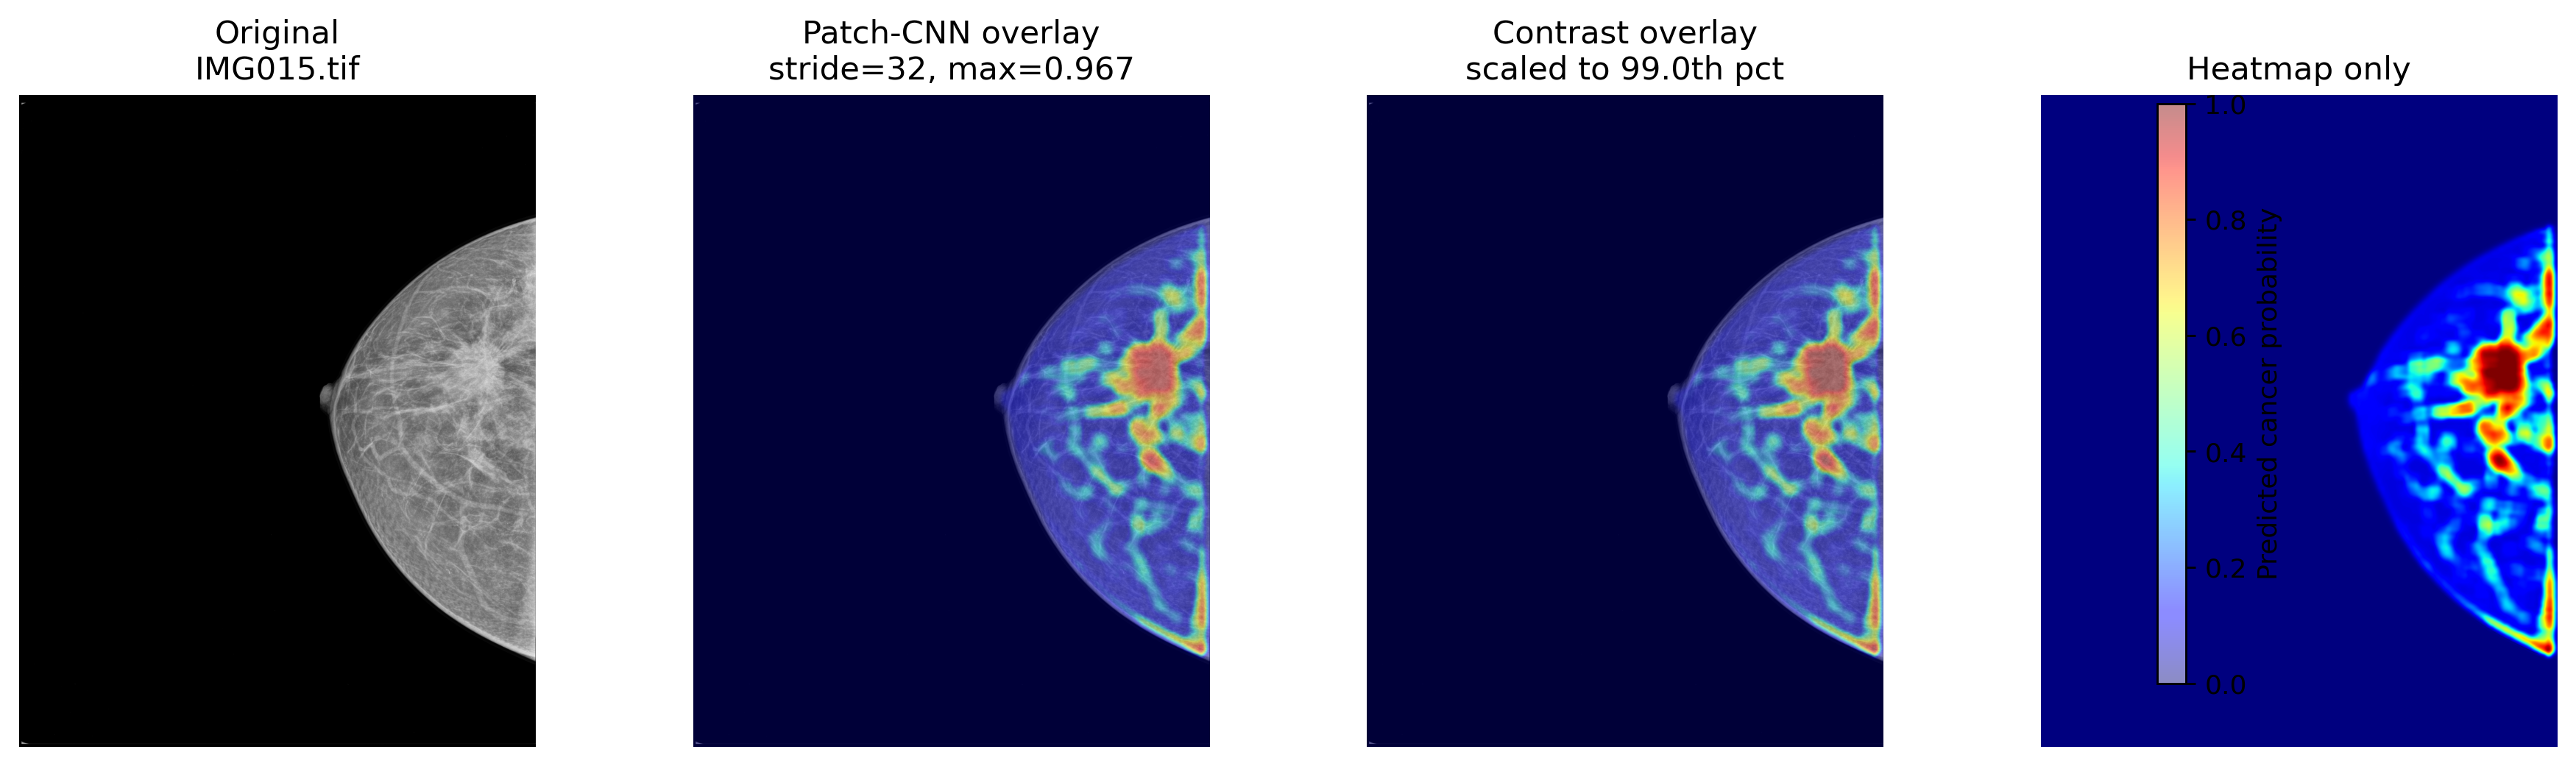
\includegraphics[width=0.82\textwidth]{../results/deep_patch_cnn/heatmaps/IMG015_patch_cnn_heatmap.png}

\vspace{0.25em}
\textbf{Single signed radial-kernel heatmap on the same image}\\[0.1em]
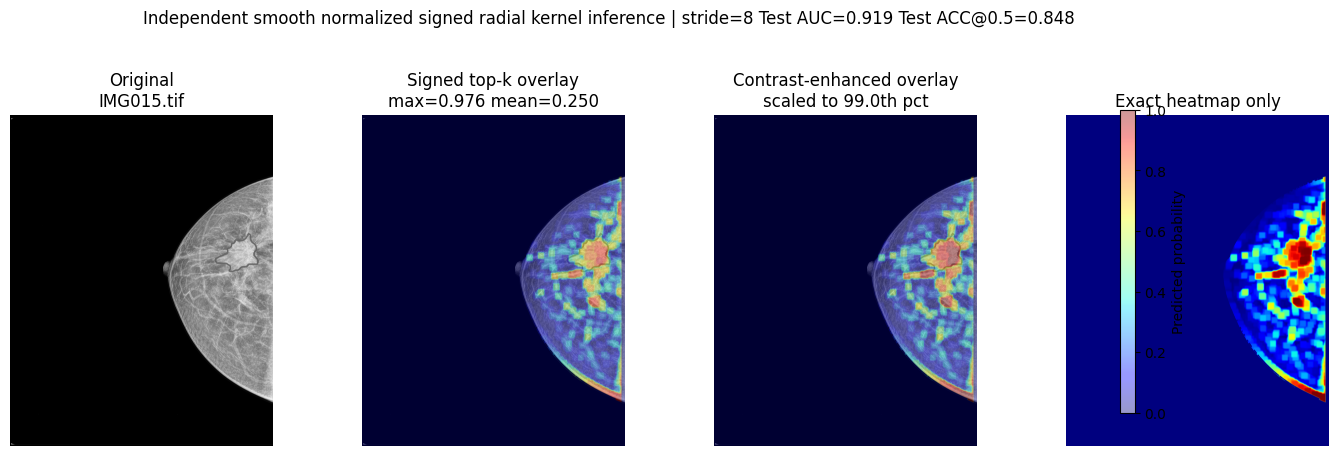
\includegraphics[width=0.82\textwidth]{figures/radial_kernel_from_scratch_heatmap.png}
\end{center}

\section*{Next Steps}

\begin{itemize}
    \item Tune the heatmap stride and smoothing to make the full-image visualization less blocky while keeping localization sharp.
    \item Add threshold tuning or calibration if the heatmap probabilities are used quantitatively instead of only visually.
    \item Finalize Resnet implementation as a second deep-learning baseline.
\end{itemize}

\end{document}
